%!TEX root = ../crimson_throne_book_main.tex
% 2014-08-02
\section{15 Sarenith 4708}

Just like the coronation three days ago Trinia's execution takes place on the terrace of the Castle overlooking Ramp Boulevard. Once more the toast of Korvosa is in attendance, for a more macabre show this time.\hyperref[fig:Quint-and-his-friends-witness-the-execution-470603218]{ Quint and his friends are among these honored guests } and, although they seriously doubt that justice is being served today, they don't see how they can stop the event. An impressive host of Gray Maidens stands guard, using their wall of silver shields to keep the visitors back. The streets below are filled with people as well, who have read about Trinia's crime and confession in today's edition of the Korvosa Herald. They do not seem to doubt the painter's confession and are eager to see her head drop. \\

\begin{figure}[h]
	\centering
	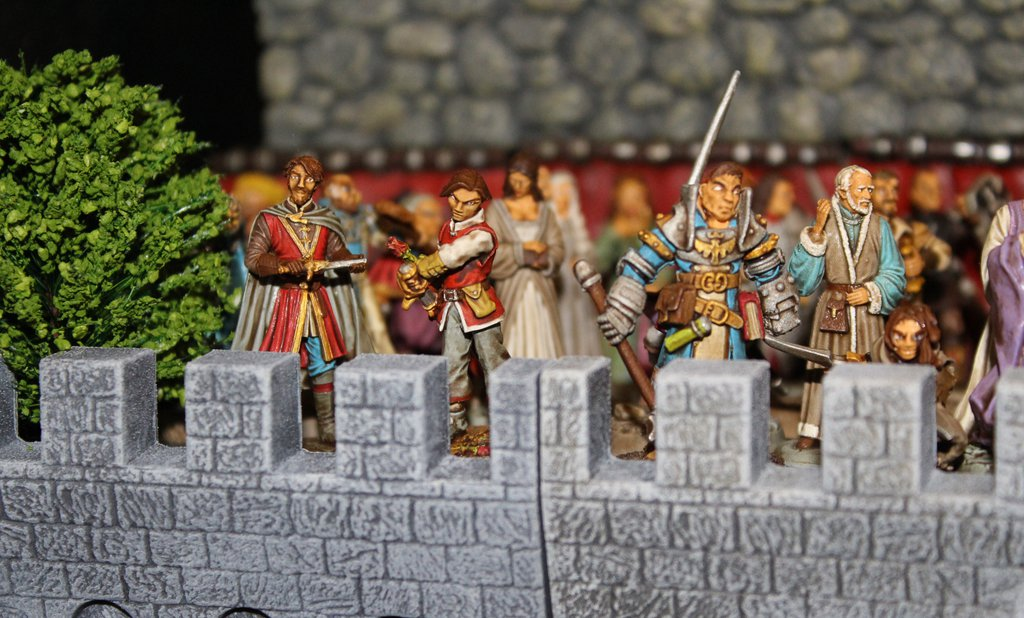
\includegraphics[width=0.39\textwidth]{images/Quint-and-his-friends-witness-the-execution-470603218.jpg}
	\caption{Quint and his friends witness the execution}
	\label{fig:Quint-and-his-friends-witness-the-execution-470603218}
\end{figure}

Drums roll as the queen emerges from the castle, closely followed by her bodyguard shadow Sabina Merrin. Having fully accepted the mantle of monarch, Ileosa carries herself with a graceful pride, showing off her beauty in a magnificent gown of green and white silk. The icy glare in her eyes totally ignores the elite that has gathered on the terrace. In her wake follows a towering, muscular man with a hood covering his face and an enormous axe in his hand. The drums suddenly change their beat to a more ominous tune as a young manacled girl with a bag over her head is herded out of the castle. Gray Maidens deliver her to the executioner's block, before pulling away the bag to reveal a\hyperref[fig:Trinia-Sabor-facing-the-executioner-470603042]{ frightened woman } who can barely keep back her tears. While one of the soldiers unlocks the shackles, another pulls back Trinia's hands and binds them behind her back with a leather cord. Then she forces the girl to her knees, her head looming over the block. \\

\begin{figure}[h]
	\centering
	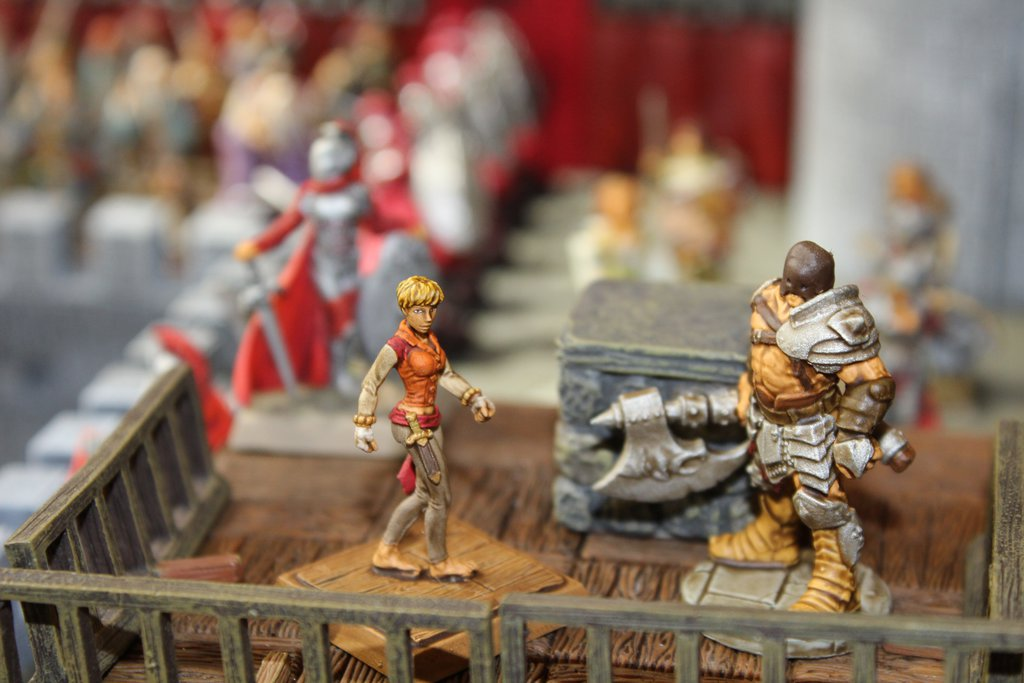
\includegraphics[width=0.39\textwidth]{images/Trinia-Sabor-facing-the-executioner-470603042.jpg}
	\caption{Trinia Sabor facing the executioner}
	\label{fig:Trinia-Sabor-facing-the-executioner-470603042}
\end{figure}

\hyperref[fig:The-execution-of-Trinia-Sabor-470602177]{ Ileosa walks over to the podium } overlooking the crowd and addresses her subjects: "Fellow Korvosans. The past few weeks have been hard on all of us. We have suffered greatly under the sea of trouble that washed over our city. I feel your suffering, for not only have I lost a beloved husband, but with each riot, each burning home, each act of anarchy and each victim my heart bled a little more. This has been a trying time for us, yet your torment is at an end. \\

\begin{figure}[h]
	\centering
	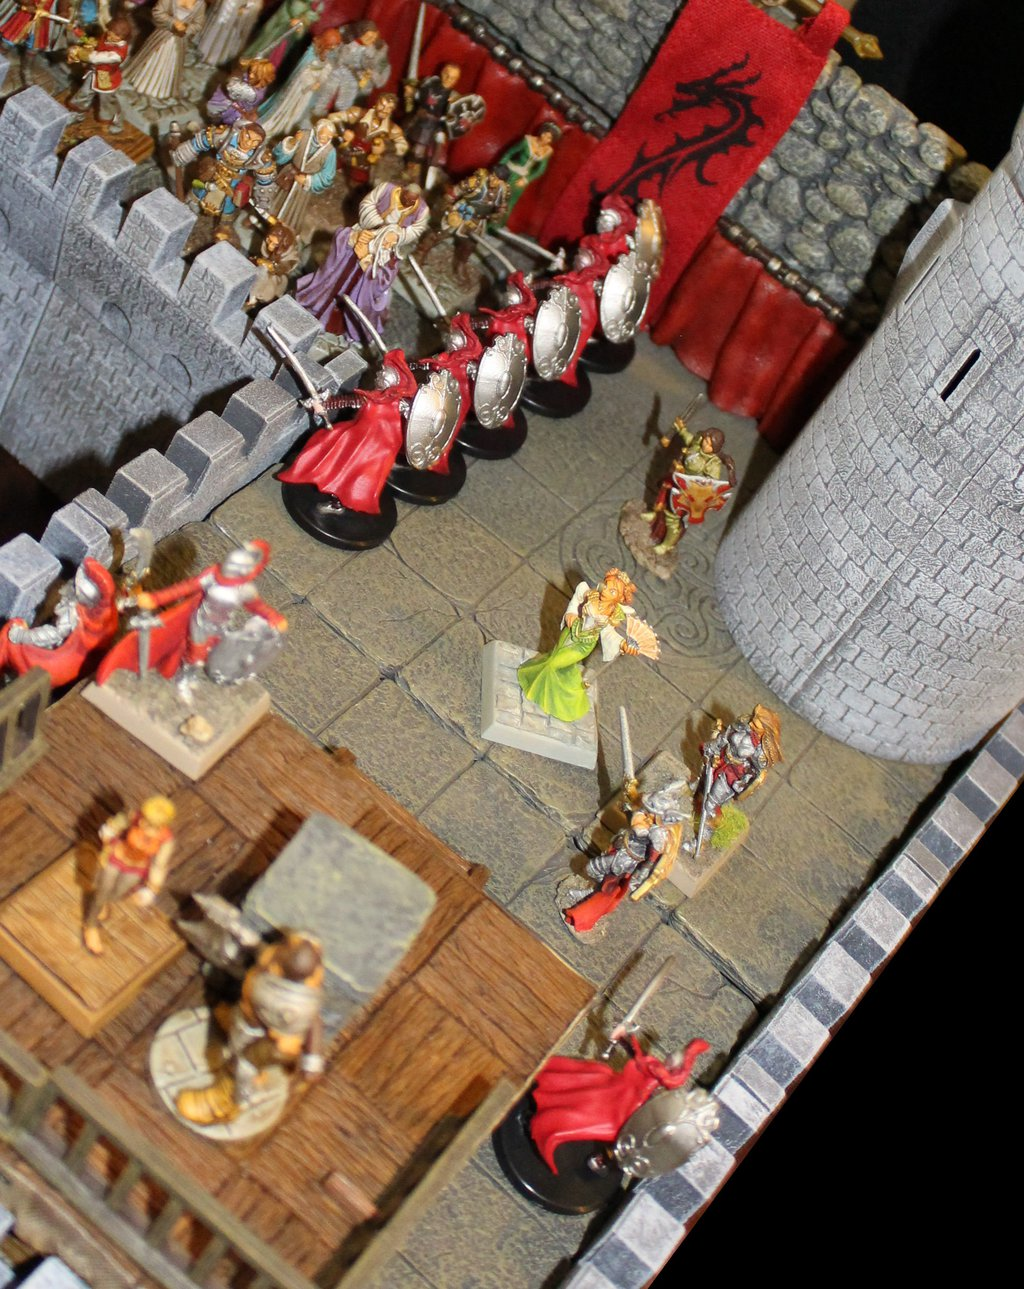
\includegraphics[width=0.39\textwidth]{images/The-execution-of-Trinia-Sabor-470602177.jpg}
	\caption{The execution of Trinia Sabor}
	\label{fig:The-execution-of-Trinia-Sabor-470602177}
\end{figure}

Before you is the cause of all this misery. Do not be deceived by her innocent nature - she is a black-hearted assassin, a seductress and a sinner, a viper amidst us all. I offer you her head as a salve against the hatred and hurt you have suffered. Her death will not rebuild Korvosa, nor will it bring back the king. Yet tomorrow will be a new dawn - a dawn over a city ready to rise from the edge of anarchy to become stronger than ever before!\\

And so, without further ado, let us usher in this new dawn with an act us justice! Off with her head!"\\

As the headsman slowly lifts his axe overhead, the crowd freezes in anticipation. His muscles bulge under the weight of the weapon. Quint, Balian, Sjo and Puk stand only a few yards away, disheartened but unable to interfere. Just as the executioner wants to swing down his axe, he gives a grunt and staggers. He lowers his weapon, reaching with his left hand to the small of his back, which is hidden from the spectators on the terrace. When he brings his hand to his face, the companions see that his fingers drip with blood. Puk then notices the flash of a slender dagger through the air that embeds itself in the headsman's right hand, forcing him to drop his weapon. Trinia raises her head, glancing up at the executioner who doubles over in pain, now revealing his first source of pain: a throwing dagger in his back. A scream echoes through the crowd: "By the Gods, it's Blackjack!"\\

From the towers of the Castle, swinging at the end of a slender crimson banner, a cloaked figure sails through the air and lands on the podium between Trinia and the axeman. As his feet touch the block where the young painter's head was meant to be separated from her body, his rapier flashes forward, slashing through the bonds on Trinia's wrists. While the girl rises to her feet, the\hyperref[fig:Blackjack-rescues-Trinia-Sabor-472558046]{ masked crusader } shouts: 'Yes indeed, Queen Ileosa! Let us usher in a new dawn with an act of justice - but true justice, not this deceit with which you try to blind Korvosa!" \\

\begin{figure}[h]
	\centering
	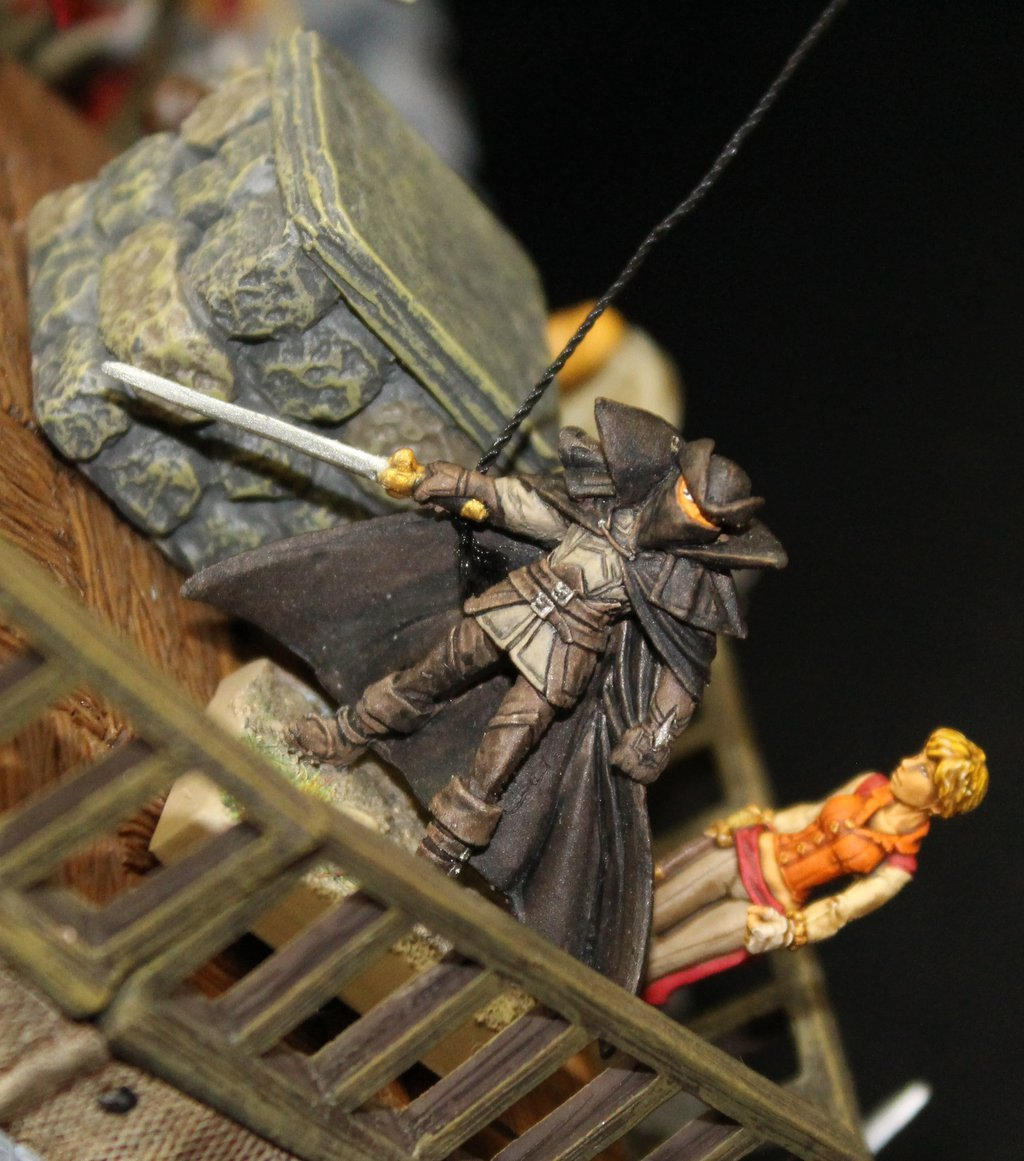
\includegraphics[width=0.39\textwidth]{images/Blackjack-rescues-Trinia-Sabor-472558046.jpg}
	\caption{Blackjack rescues Trinia Sabor}
	\label{fig:Blackjack-rescues-Trinia-Sabor-472558046}
\end{figure}

Everyone stands stunned for a moment. Then several onlookers burst into action at the same time. The queen whispers something to Sabina Merrin who quickly orders her troops to seize the assailant. Quint sees no path through to crowd and yells out words of discouragement to the Gray Maidens, using bluff to disguise his {\itshape satire} as a warning to be cautious of this skilled killer. Being a  {\itshape clumsily} brings down two female soldiers who were about the charge Blackjack and apologizes profusely, as he is  {\itshape only trying to help} . Meanwhile the executioner has regained his bearings and picked up his axe again, threatening to strike Blackjack from behind. Yet it seems like the cloaked scoundrel has eyes in the back of his head, for he jumps over the axeman's deadly chop before he quickly \hyperref[fig:Blackjack-saves-Trinia-Sabor-2-472559200]{ grabs Trinia by the arm } , ordering her to hang on. The next moment the caped crusader sails through the air again on the crimson banner with the young woman clinging to his side, first swinging back to the castle, then running over the wall to gain extra speed. As he swerves back down, he pushes off, propelling himself and his proxy to the roof of a nearby building. He glides off the tiles, but somehow manages to halt his momentum and regains his feet. Once more he looks up at the castle to see the queen flee inside. He raises his rapier in salute to the crowd on the terrace and in the streets (and possibly to the companions who aided his escape). With a swoop of his cloak he turns around and disappears with Trinia over the rooftops. \\

\begin{figure}[h]
	\centering
	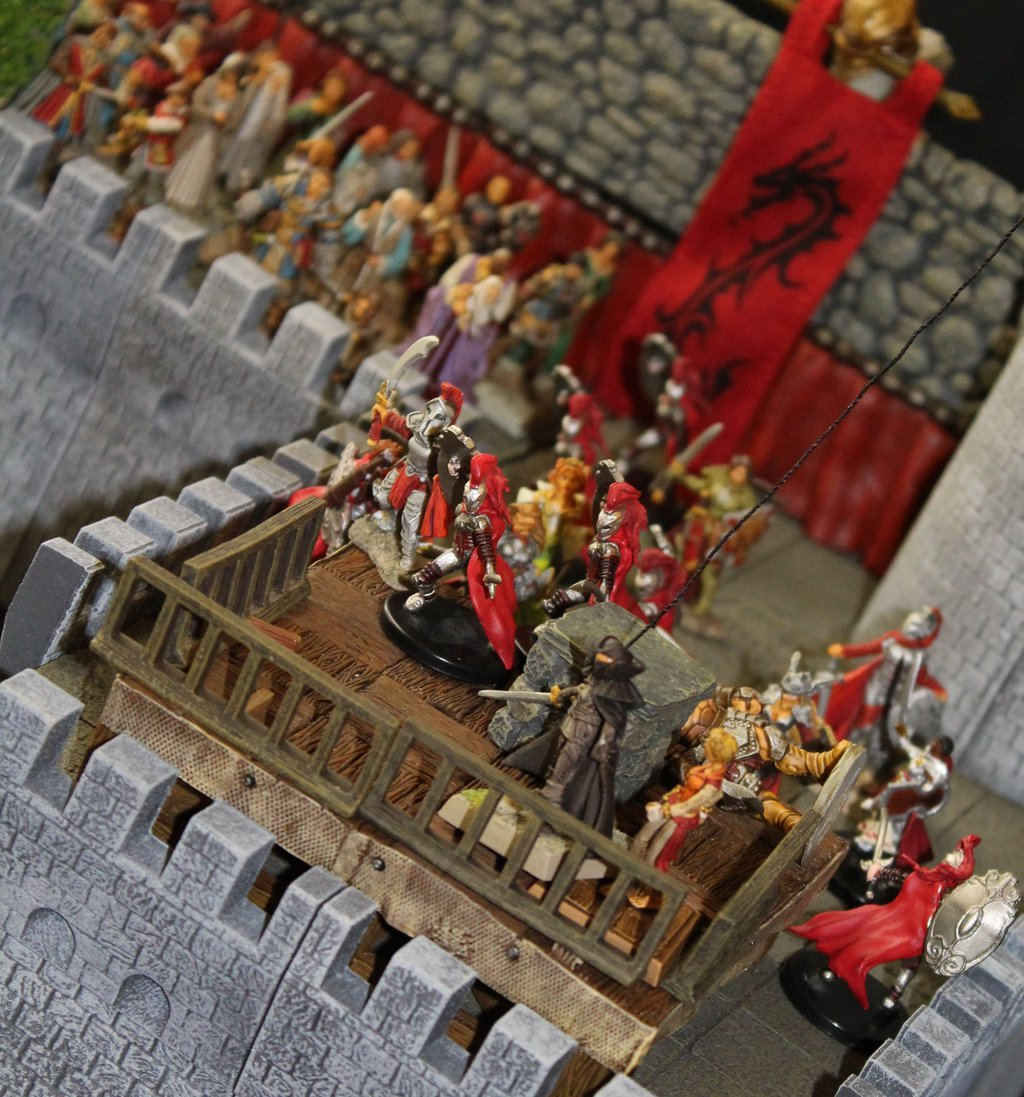
\includegraphics[width=0.39\textwidth]{images/Blackjack-saves-Trinia-Sabor-2-472559200.jpg}
	\caption{Blackjack saves Trinia Sabor 2}
	\label{fig:Blackjack-saves-Trinia-Sabor-2-472559200}
\end{figure}

Meanwhile the Gray Maidens push back the elite visitors on the terrace, ordering them to go home and showing no respect for the station of the people in front of them. Quint makes an effort to reach the executioner, offering to heal the man's wounds, but he gets driven back with the rest of the guests. He decides not to push his luck, realizing that Trinia is safe for now, and follows the aggravated nobles and dignitaries down the steps of the great mastaba that supports Castle Korvosa.\\

The companions head directly to Trinia's apartment and her friend Nisha's flat to see if either of the women are there, but find both places empty, which does not come as a big surprise. The streets in the city are filled with people who are flabbergasted by the spectacle that just transpired. Most citizens question Blackjack's motives and harbor little sympathy for his reckless rescue, as formidable a feat as it may have been. It feels like rest or peace are just not in Korvosa's cards. The Gods only know what will happen next ...\\

